\chapter{Structural Optimization}
\label{ch:struct_opt}

    
The following chapter describes the various procedures used to determine an average description of the geometry of extra-framework water molecules as a function of fill, relative angle (with respect to other water molecules), and rotation about the high-symmetry point. First, the volume of the supercell is optimized through a Birch-Murnaghan equation of state fitting in Section \ref{sec:eos}. Then, an assumption implemented in existing studies is tested in Section \ref{sec:da} (i.e. decoupling of the water molecule from the beryl framework) before internal relaxations of the supercell are carried out in various configurations in Section \ref{sec:geo_opt}.

For each of the three sub-processes mentioned above, relevant background information, procedures, computational details, and analyses are provided. As each sub-process builds upon the previous' results, the final results and conclusions of this chapter are highlighted at the end of Section \ref{sec:geo_opt}.
    
    \section{Equation of State Fitting}
    \label{sec:eos}
        
            An equation of state describes the relationship between thermodynamic properties of a system. For instance, the Birch-Murnaghan equation of state, as described in detail in \textbf{[CITE: ((bmeos)) PRB 70,224107]},
            
            \begin{equation}
            \label{eq:bm_eos}
                E(\eta) = E_0 + \frac{9B_0V_0}{16}\left(\eta^2 -1\right)^2\left[ B'_0 \left(\eta^2-1\right) -4\eta^2\right] \text{ with } \eta = \left(\frac{V}{V_0}\right)^{1/2}
            \end{equation}
            
            \noindent relates the optimum volume $V_0$, the bulk modulus $B_0$, the first derivative of the bulk modulus $B'_0$, and the energy of the system $E$ as a function of current volume $V$. (Or, rather here, the square-root of the normalized volume $\eta$ is used.)
            
            Equation \ref{eq:bm_eos} suggests a technique for determining the aforementioned thermodynamic quantities by calculating the energy of a system at various scaled volumes, which is outlined below.
            
        \paragraph{Procedure} The following is a general procedure for fitting any equation of state, such as Eq. \ref{eq:bm_eos}. First, an initial "guess" structure $\sigma_g$ is acquired, typically from theory or experiment, with volume $V_g$. Using this structure, an ensemble of structures $\sigma_i$ with volume $V_i$ are constructed such that
        
        \begin{equation}
        \label{eq:ensem_eos}
            V_i \in \{ V_i : (1-x)V_g \le V_i \le (1+x) V_g \},
        \end{equation}
        
        \noindet for $0<x<1$. The initial structure $\sigma_g$ should be such that the set $\{V_i\}$ corresponds to volumes in the neighborhood of $V_0$. Using each corresponding structure, the energy $E_i(V_i)$ is calculated via a self-consistent DFT run. Finally, the resulting data is fit to Eq. \ref{eq:bm_eos} and the relevant optimized parameters are extracted.
        
        For the beryl-water system, the set of $\{ V_i\}$  is constructed by varying the lattice constants $a$ and $c$ over a range around the known values. (Technically, only $a$ is varied, since the relationship (\ref{eq:c_a}) between it and $c$ is known.) This process occurs in two steps: (a) coarse-grain scan and (b) fine-grain scan. For the coarse-gran scan, lattice constant $a$ is investigated over $8.7 \le a \le 9.6$ $\angstrom$ and $\Delta a = 0.1$ $\angstrom$. After a preliminary analysis, a smaller range is investigated in the fine sweep---specifically, $9.20 \le a \le 9.38$ $\angstrom$ with $\Delta a=0.01$ $\angstrom$. For each lattice constant, the volume is calculated according to 
            
        \begin{equation}
        \label{eq:c_a}
            V(a) = \frac{\sqrt{3}}{2} a^2 c \text{ with } \frac{c}{a} = 0.998
        \end{equation}
        
        \noindent for beryl.
        
        \paragraph{Calculation Details} The standard self-consistent calculator as outlined in Section \ref{sec:calc_details} is employed for all self-consistent calculations. 
            
        
        
        \begin{figure}
            \centering
            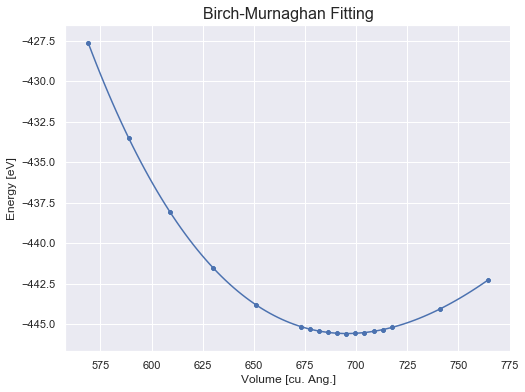
\includegraphics[width=0.8\linewidth]{Figures/System/eos.png}
            \caption{The calculated energies $E_i(V_i)$ are shown with the accompanying Birch-Murnaghan equation of state fit. The optimized volume is $V_0=695.39$ \angstrom$^3$. See text for literature comparison.}
            \label{fig:eos_fit}
        \end{figure}
        
        \begin{table}[]
            \centering
            \begin{tabular}{c|c|c}
                Observable & Value & Experiment \textbf{[CITE: eosfit]} \\
                \hline
                \hline
                $V_0$ [\angstrom$^3$] & 695.39 & $675\pm0.1$ \\
                $B_0$ [eV/\angstrom$^3$] & 1.1249 & $1.1 \pm 0.01$ \\
            \end{tabular}
            \caption{The optimized volume and bulk modulus as extracted from the fit in Fig. \ref{fig:eos_fit} are compared to literature values. See text for analysis.}
            \label{tab:eos_compare}
        \end{table}
        
        \paragraph{Results and Analysis} Figure \ref{fig:eos_fit} shows the calculated equation of state, along with the fit and comparison to literature values (see Table \ref{tab:eos_compare}). The calculated optimized volume of $V_0 = 695.39$ \angstrom$^3$ is in good agreement with the literature value of $V=675\pm0.1$ $\angstrom^3$, especially considering that the literature values are determined at ambient temperature and pressure. 
        
        It is worth noting that investigating the effects of different functionals, pseudopotentials, basis sets, etc. could yield results closer to the literature value, but reproducing nature exactly is not the point of this study. Rather, an attempt is being made to develop a protocol for efficiently parameterizing force fields for extra-framework water. Furthermore, the desire to settle discrepancies in literature, specifically with regards to the potential map, necessitate the choice of functional and pseudopotential.
        
        Moving forward, the cell volume will be fixed to $V=695.39$ $\angstrom^3$.
    \section{Decoupling Assumption}
    \label{sec:da}
        \paragraph{Background Information} As previous work has demonstrated, there is no appreciable difference in geometry, potential map, or vibrational spectra in terms of different exchange-correlation functionals, both with and without dispersion corrections \cite{vibr_states}. Effectively, this allows the crystal framework to be viewed as producing a static potential well in which the extra-framework water molecules interact. However, this assumption has been made in cases in which the electronic subsystem of the water molecules (i.e. dipole moment) is excluded from investigation. Therefore, while this assumption is definitely ideal in terms of the computational cost of converging over 400 ions and electrons in the beryl unit cell, it needs to be explicitly tested if it is to be used during the geometry optimization. 
            
        \paragraph{Procedure} To begin, a single water molecule is added to the unit cell of beryl in the standard position. Such a system has a fill factor of 50\%. For each energy difference stopping tolerance (EDST), positional degrees of freedom for both beryl and the water molecule ions are allowed to relax---this is referred to as the \textit{full} relaxation. Then an independent, second relaxation is performed in which the beryl ions are held fixed, and only the water molecule ions are allowed to relax---this is referred to as the \textit{selective} relaxation.
            
        To compare the two relaxation schemes, the difference in position of each ion between the full and selective relaxations are calculated. By looking at both the average displacement and the maximum displacement between ions, the validity of the decoupling assumption can be determined. Additionally, the average of the water molecule bond lengths and the OHO-angle are compared for both schemes. Again, assuming the decoupling assumption holds, there should be no appreciable difference in the geometry parameters of the water molecule.
            
        \paragraph{Calculation Details} For both the full and selective relaxation, the relaxation calculator is used. The relaxations are performed with EDST os $10^{-4}$ and $10^{-5}$. After both relaxations have been performed for each EDST, the Atomic Simulations Environment (ASE) \textbf{[CITATION]} is used to calculate the difference in ionic positions $\Delta r_i$ for each ion $i$. From the set of all ionic position differences $\{\Delta r_i \}$, the average displacement $\langle \Delta r \rangle$ and maximum displacement $\Delta r_\text{max}$ are determined. Additionally, the average OH bond length $\langle r} \rangle$ and the OHO angle $\theta$ of the water molecule are determined for both relaxation schemes.
            
        To test the convergence of the geometry optimization results, the ratios of the water geometry parameters $\langle r \rangle$ and $\theta$ for EDST are calculated, with a ratio near unity indicating that there is no significant difference in geometry with respect to the EDST. Once convergence is established, the ratios of the average OH bond $\langle r \rangle$ and OHO angle $\theta$ for the full and selective relaxations are compared, again with a ratio near unity indicating that the decoupling assumption holds.
        
        
        
        
        \begin{figure}
             \centering
             \begin{subfigure}[t]{0.45\textwidth}
                 \centering
                 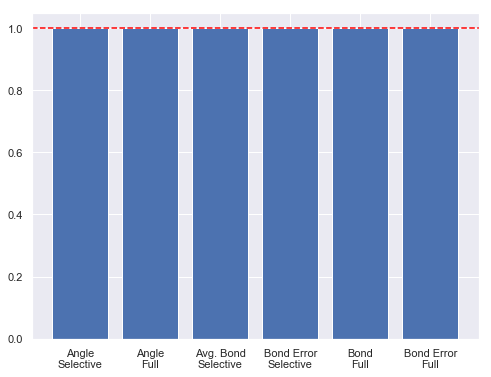
\includegraphics[width=\textwidth]{Figures/System/ediff_geom_ratios.png}
                 
                 \label{fig:ediff_geom_ratios}
             \end{subfigure}
             \hfill
             \begin{subfigure}[t]{0.45\textwidth}
                 \centering
                 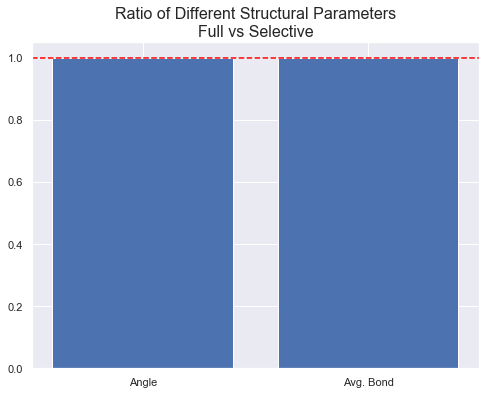
\includegraphics[width=\textwidth]{Figures/System/selective_v_full_geom_params.png}
                 \label{fig:selective_v_full}
             \end{subfigure}
                \caption{Decoupling assumption results. The red, dashed line denotes unity. (Left) The ratio of certain geometry parameters (and associated errors where appropriate) as calculated under energy difference tolerances $10^{-4}$ and $10^{-5}$. (Right) The ratio of OHO angle and average of the two OH bond lengths for the water molecule under the full and selective relaxation schemes with energy difference tolerance of $10^{-4}$. See text for full analysis.}
                \label{fig:decouple_assumption}
        \end{figure}
        
        \paragraph{Results and Analysis} The decoupling assumption results are summarized in Fig. \ref{fig:decouple_assumption}. Starting with the left sub-figure therein, it is clear that there is no measurable difference between the relevant geometry parameters in terms of energy stopping tolerance. Specifically, the ratio of each observable is nearly unity. It is therefore reasonable to conclude that the larger EDST of $10^{-4}$ produces converged structures.
        
        \begin{table}[]
            \centering
            \begin{tabular}{c|c|c}
               Tolerance  & $\langle \Delta r \rangle$ & $\Delta r_\text{max}$  \\
               \hline
               \hline
                $10^{-4}$ & $0.008\pm 0.001$ & $0.031$  \\ 
                $10^{-5}$ & $0.010\pm0.001$& $0.033$ \\ 
            \end{tabular}
            \caption{The average difference in position over each ion and maximum difference in position between the two relaxation schemes for different energy difference tolerances. All distance measurements are in Angstroms.}
            \label{tab:ediff_r_diff}
        \end{table}
        
        Looking at the right subfigure in Fig. \ref{fig:decouple_assumption}, the average OH bond length $\langle r \rangle$ and OHO angle $\theta$ for both the full and selective relaxations with EDST $10^{-4}$ are compared via their ratios. Again, the ratios of both geometry parameters are nearly unity, suggesting there is no significant difference in the water molecule geometry between the two relaxation schemes. Furthermore, as shown in Table \ref{tab:ediff_r_diff}, both the average displacement and maximum displacement of the ions under the two relaxation schemes is significantly small compared to the length of the lattice vectors ($<1\%$ in both cases). 
        
        The validity of the decoupling assumption is therefore confirmed for purposes of geometry optimization under an EDST of $10^{-4}$ eV.
        
        
    \section{Water Geometry vs. Fill, Relative Angle, Rotation}
    \label{sec:geo_opt}
    
    With the validity of the decoupling assumption and corresponding selective relaxation scheme established, the geometry of the water molecules can be determined as a function of fill, relative angle with respect to other water molecules, and rotation about the high-symmetry point. Specifically of interest are the OH bond length $r$ and OHO angle $\theta$ and how they change, if at all. Do these geometric parameters have a well-defined, meaningful average value? Do the water molecule geometries change when more molecules are present? How do these parameters vary when the relative angle between extra-framework water molecules change? Does the interaction between framework and extra-framework species have any effect on the geometry of said extra-framework species? The remainder of this chapter sets out to answer these questions.
    
    
    \begin{figure}
        \centering
        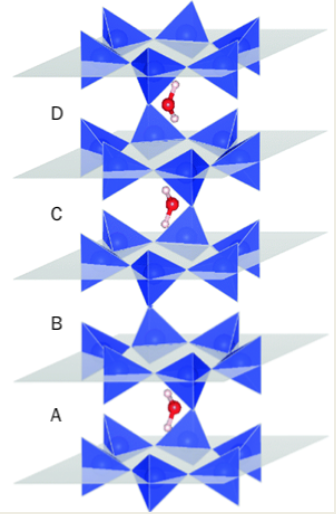
\includegraphics{Figures/System/geometry_supercell.png}
        \caption{Depiction of the supercell, with labeled cages A-D, used for the geometry optimization as outlined in the text. [\textbf{Adapted from 10.1039/c7cp06472a}]}
        \label{fig:geom_supercell}
    \end{figure}
    
    \paragraph{Procedure} To start, a supercell is created by replicating the unit cell once in the c-direction, resulting in four cages, as shown in Fig. \ref{fig:geom_supercell}. The cages are labelled, starting from the bottom-most, as A, B, C, and D. With four cages, it is possible to probe fill factor $\phi \in \{0.25,0.50,0.75,1.00 \}$. For $\phi=0.50$, there exists a degeneracy in the fill configurations, i.e. both configurations with A \& C filled and A \& B filled correspond to the same fill factor. To make discussion herein as unambiguous as possible, the binary conventions in Table \ref{tab:fill_conventions} are adopted throughout. Occasionally, the water molecule that occupies a cage may be referred to by the cage label. For example, in Fig. \ref{fig:geom_supercell}, the water molecule in cage C may be referred to as water molecule C. 
    
    \begin{table}[]
        \centering
        \begin{tabular}{c|c}
           Fill  & Occupied Cages \\
           \hline
           \hline
           1000  &  A \\
           1010  &  A, C \\
           1100  &  A, B \\
           1110  &  A, B, C \\
           1111  &  A, B, C, D\\
        \end{tabular}
        \caption{The binary convention adopted to describe the different fill possibilities.}
        \label{tab:fill_conventions}
    \end{table}
    
    While the fill factor $\phi$ provides one dimension of the parameter space to explore, it does not encompass the entirety of the space. The geometry must also be probed as a function of relative angle to the beryl framework \textit{and} the relative angle between extra-framework water molecules. Naturally, only a small subspace of this parameter space can be sampled, and said subspace is outlined in Table \ref{tab:param_subspace}.
    
    For example, for fill 1110, molecule C is held fix, while molecule A is rotated through 12 rotations totaling $2\pi$, and for each rotation of A, molecule B is also rotates through 12 rotations totaling $2\pi$. In all, $12^2 = 144$ configurations are sampled for this fill. Also, for fill 1111, molecules A-C and B-D are pairwise ferroelectrically coupled, and therefore rotate together. 
    
    The above demonstrates the difficulty of adequately sampling this parameter space, especially considering the expense of these calculations (approximately eight hours per configuration with the available resources). Given more resources, a greater sample size would be ideal, specifically increasing the number of rotations. It may also help optimization if the rotation angle were decreased to encompass only the asymmetric unit of the crystal rather than a full $2\pi$ rotation.
    
    In addition to performing the above procedure with the water molecules in the beryl framework, the calculations are also performed without the beryl atoms. In other words, the spacing and rotation of the water molecules is the same, but the calculations are carried out in vacuum. This allows for investigation of how the beryl framework affects the geometry, if at all.
    
    \begin{table}[]
        \centering
        \begin{tabular}{c|c|c|c}
            Fill & No. Rotations & Rotation Angle  & Rotated Molecules  \\
            \hline
            \hline
            1000 & 30 & $2\pi$ & A \\
            1010 & 12 & $2\pi$ & A, C \\
            1100 & 12 & $2\pi$ & A, B \\
            1110 & 12 & $2\pi$ & A, B \\
            1111 & 12 & $2\pi$ & A-C,B-D \\
        \end{tabular}
        \caption{Outline of the parameter subspace sampled as part of the geometry optimization. See text for details.}
        \label{tab:param_subspace}
    \end{table}
        
        \paragraph{Calculation Details}
        
        For each configuration in Table \ref{tab:param_subspace}, the selective relaxation scheme as outlined in \ref{sec:da} is used. After the relaxation, the relevant geometric measurements are made using ASE. 
        
        \paragraph{Results and Analysis}
        \label{sec:geom_opt}
        
        \begin{figure}
            \centering
            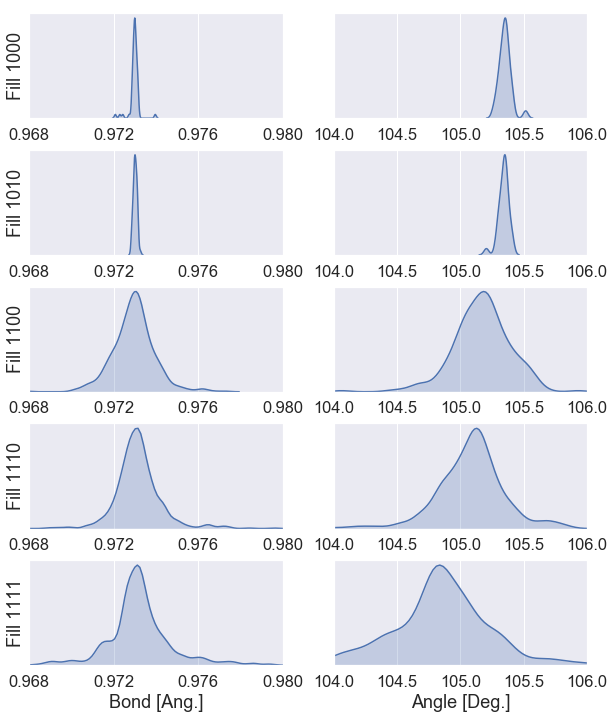
\includegraphics[width=0.85\linewidth]{Figures/System/geom_kdes.png}
            \caption{Kernel density estimates for the OH bond lengths (left) and OHO angles (angles) by fill for water molecules in beryl. }
            \label{fig:geom_kdes}
        \end{figure}
        
        Figure \ref{fig:geom_kdes} shows the kernel density estimates for the OH bond length and OHO angle populations for the in-beryl case. Each subplot represents the population density of the sampled set. Immediately clear is the fact that there is an effect of fill on the geometry of the water molecules, as evident by the qualitative difference in shape of the population densities. For each, there is a well-defined peak, suggesting that an average geometry per fill is meaningful. However, the variance of the population density is directly proportional to the fill, suggesting that rotation does have some effect on the geometry with the effect being more prominent for greater fills. 
        
        
        
        \begin{figure}
            \centering
            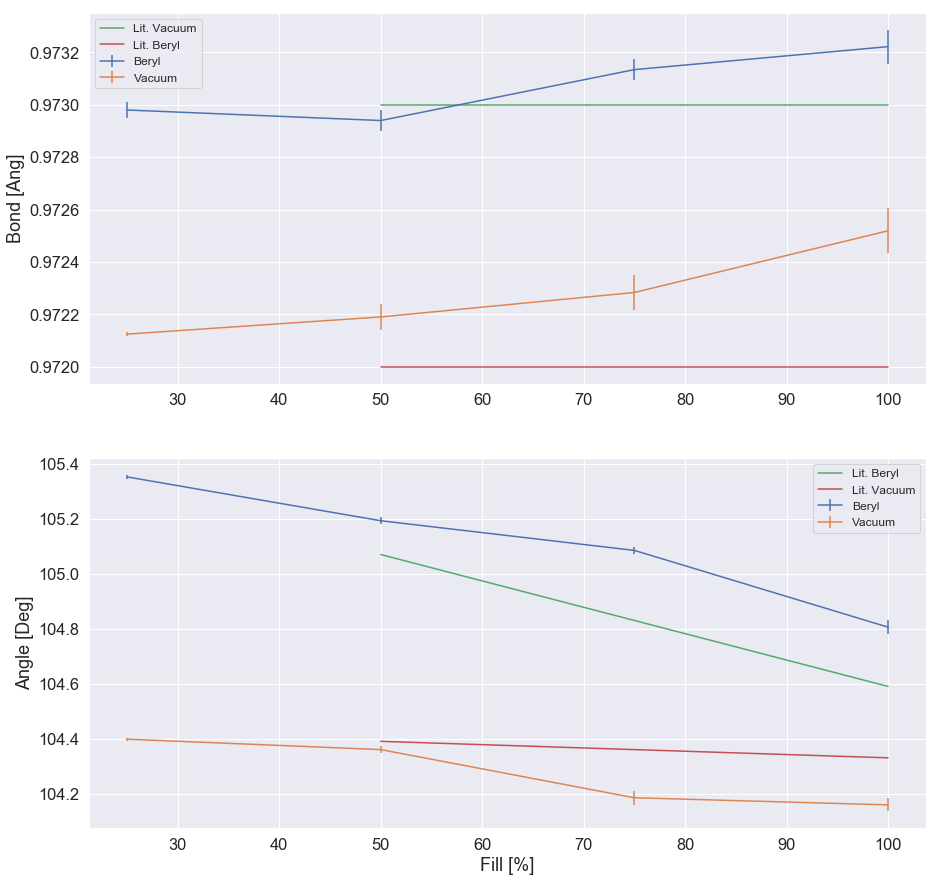
\includegraphics[width=0.85\linewidth]{Figures/System/geom_results.png}
            \caption{The average OH bond length (top) and OHO angle (bottom) per fill factor are compared to literature values, when possible. Error bars represent the standard errors of the mean.}
            \label{fig:geom_results}
        \end{figure}
        
        For a more quantitative analysis, the averages and standard errors of the mean are used as shown in Fig. \ref{fig:geom_results}. Here, the populations (and therefore, results) for fills 1010 and 1100 are combined. 
        
        From both the OH bond length and OHO bond angle (blue line), it is clear that there is an effect from the fill factor on the geometry of the water molecule. Specifically, as more water molecules are added, the OH bond lengthens slightly, while the OHO angle decreases. Additionally, an effect from the beryl crystal is evident (orange vs. blue line) in that the beryl has a \textit{dilating} influence on the water molecule---the OH bond length systematically increases and the OHO angle systematically expands. 
        
        As a benchmark, these results are acceptably compared to the work done in \cite{vibr_states} (green and red lines). Here, the systematic differences can be explained by the procedure followed in said work. Instead of relaxing the water molecule under the optimized beryl geometry, the beryl geometry was set to match an experimental sample to which they were comparing their computational results. Additionally, only fill factors $\phi = 0.50, 1.00$ were investigated. 
        
        Moving forward, the fill specific geometries, as shown in Fig. \ref{fig:geom_results}, are used. 
        
    \section{Summary and Outlook}
    
    In Section \ref{sec:eos}, the well-behaved energy versus volume curve yielded an optimized volume of $V_0 = 695.39$ $\angstrom^3$, which is within 3\% of the literature value as measured at STP. The calculated bulk modulus $B_0 = 1.1249$ eV/$\angstrom^3$ is just outside the experimental margin of error ($B_{0,\text{exp}} = 1.1 \pm 0.01$ eV/$\angstrom^3$). While results are in good agreement with literature, improvements could be made by either fitting to more than just the Birch-Murnaghan equation of state and averaging the optimized thermodynamic properties from each fit, or different functionals or pseudopotentials could be tested to determine their effect. 
    
    After performing the geometry optimization under both the full and selective relaxation protocols for EDST $10^{-4}$ and $10^{-5}$ in Section \ref{sec:da}, the larger tolerance and selective relaxation protocol are deemed appropriate, since no significant difference is measurable. In the future, testing this assumption with a smaller EDST and/or more water molecule configurations will either reaffirm the findings here or suggest more accurate approximations.
    
    Finally, geometry optimization of the extra-framework water molecules is carried out in Section \ref{sec:geo_opt}. A measurable effect on geometry as a function of fill is observed. Specifically, the OH bond length increases slightly with fill, while the OHO angle decreases slightly. The geometry optimization was also carried out in vacuum (without the beryl framework but with the same spacing of extra-framework water molecules), and similar trends were observed. A systematic increase in both OH bond length and OHO angle was observed when moving from the vacuum to in-beryl case, suggesting that the framework crystal exerts a dilating effect on the water molecule.
    
    In retrospect, some significant improvements in this protocol are apparent. Mainly, the water molecule configurations coincided symmetry points with respect to the framework crystal. By increasing the rotational sample frequency, less symmetric configurations would be sampled. Even better, a random, Monte Carol-esque method for selecting the rotation angles between framework and extra-framework molecules would provide for a more efficient sampling of this parameter space. Additionally, it would be interesting to see what happens if the degrees of freedom for the water ions was limited in such a way that the ions can only move within the OHO-plane. This would force the water molecule to retain its angle relative to the framework, which is not currently the case.
        
    To improve upon these parameters, a larger subspace of the parameter space should be investigated. Additionally, changing the size and shape of the unit cell---and thus the fill configurations that correspond to certain fill factors $\phi$---and investigating the average geometry would be of interest. Notably, what happens if the supercell is created by replicating the unit cell along the a- or b-directions? 